\chapter{Usability Test}\label{ch:outlook}

Aufbauend auf allen bisher getätigten Analysen und Anpassungen des Interface, gilt es abschließend noch den Prototypen und die Implementierung mithilfe eines Usability Tests zu evaluieren.
Hierbei wird im Schritt \glqq Finalize the UX design\grqq{} des Human-Centered Design Process die Rolle des Usability Testers abgedeckt, welcher für die Durchführung der Auswertung des Usability Tests zuständig ist.
Auf weitere Anpassungen des Interface wird verzichtet.

In diesem abschließenden Kapitel werden die Grundlagen des verwendeten Tools für den Usability Test erläutert.
Darauf folgend wird die Art des durchgeführten Tests definiert und dargelegt auf welchen Grundlagen diese Wahl getätigt wurde.
Aufbauend auf den theoretischen Erläuterungen wird die letztendliche Testaufgabe konkret definiert und die nötigen Anweisungen, sowie die Materialien zur Auswertung der Tests erstellt.
Abschließend werden die Ergebnisse der durchgeführten Auswertungen der Tests dargestellt und interpretiert, bevor es einen Ausblick auf das mögliche weitere Vorgehen gibt.

\section{Lookback}

Bei Lookback handelt es sich um eine Cloudbasierte Softwarelösung, die es ermöglicht User Experience geräteübergreifend zu dokumentieren.
Bei der Durchführung der Tests besteht die Möglichkeit, als Tester aktiv teilzunehmen oder die Probanden unmoderiert mit dem Prototyp oder der Software interagieren zu lassen.
Möchte der Usability Tester teilnehmen -  also einen \glqq In Person\grqq{} Test durchführen - kann aus den beiden Möglichkeiten gewählt werden, die Tests mit dem Nutzer innerhalb einer Live-Session oder persönlich vor Ort an einem Rechner abzuhalten.

Für die durchzuführenden Tests erstellt der Usability Tester innerhalb von Looback ein Projekt.
Zugunsten des Datenschutzes besteht hier die Möglichkeit die Projekte auf privat zu setzen und nur ausgewählten Personen des Teams Zugriff zu den Aufnahmen  der Tests zu gewähren.
Innerhalb der Projekteinstellungen können Instruktionen für die Nutzer bereitgestellt werden, die während des Tests erscheinen und durch die Aufgaben führen.
Das ist vor allem dann hilfreich, wenn die Testperson den Test autonom durchführen soll.

Sollte der Test nicht gemeinsam in einem Raum stattfinden, kann mithilfe eines Links der Test mit den Probanden geteilt werden.
Der Tester bekommt eine Benachrichtigung, sobald der Proband bereit ist bzw. mit der autonomen Durchführung begonnen hat.
Während der Session hat der Tester die Möglichkeit mit Zeitstempel versehene Notizen zu machen oder mit eventuell teilnehmenden Teamkollegen zu chatten.
Diese Möglichkeit der Live-Dokumentation erleichtert die darauffolgende Auswertung des Test erheblich, da man sofort Auffälligkeiten festhalten kann und diese in der Aufzeichnung leichter auffindbar sind.
Nach Abschluss des Tests speichert Looback die Aufnahme in der Cloud, wodurch diese für die nachträgliche Auswertung des Tests abrufbar bleibt. \cite{.10.01.2020}

Die Möglichkeit der Live-Dokumentation bildet das ausschlaggebende Argument für die Wahl des Tools, ebenfalls besteht die Möglichkeit in der hochgeladenen Aufnahme Kommentare hinzuzufügen, was die Auswertung sehr erleichtert.
Zusätzlich ist es wichtig den Test online durchführen zu können, da viele Modellierer nicht am Hauptstandort von EB beschäftigt sind, wodurch persönliches Testen nicht immer möglich ist.

\section{Remote Usability Test}
Die im vorherigen Kapitel bereits kurz benannten \glqq In Person\grqq{} Tests finden in der Regel in einem Usability Labor statt.
Dies bezeichnet einen abgeschlossenen Raum ohne Störungsquelle, der mit der benötigten Hard- und Software ausgestattet ist und in dem sich nur der Proband und der durchführende Tester aufhalten.

Bei einem Remote Usability Test wird die Arbeitsaufgabe nicht gemeinsam im Labor, sondern räumlich getrennt durchgeführt.
Hier lässt sich noch zwischen asynchronen und synchronen Tests unterscheiden.
Bei letzteren besteht, trotz der räumlichen Trennung, eine direkte Verbindung mithilfe von Webcam und Sprachübertragung, zwischen Tester und Proband.
Gleichzeitig dazu wird der Bildschirminhalt der Testperson übertragen, um es dem Tester zu ermöglichen dessen Interaktionen zu verfolgen und durch die Aufgaben führen zu können.
Durch diese direkte Verbindung ist es für den Tester ebenfalls möglich, während, oder unmittelbar nach dem Test, Fragen zu stellen.
Bei synchronen Tests besteht der Vorteil darin, mit geringem Aufwand örtlich weit verteilte Nutzer in den Test einbinden zu können.
Zusätzlich dazu findet der Test in der gewohnten Umgebung des Nutzers statt, es wird also keine unnatürliche Situation in einem Labor geschaffen, was die Nervosität der Nutzer eventuell steigern könnte.
Auch können die Probanden hier mit ihrer gewohnten Hard- und Software arbeiten, was vor allem für repräsentative Werte, die die Effizienz betreffen, von Vorteil ist.
Durch den Umstand der gewohnten Arbeitsumgebung entsteht jedoch in vielen Fällen auch ein technischer Zusatzaufwand aufseiten des Nutzers.
So kann beispielsweise ein Headset und eine Webcam benötigt, oder zusätzliche Software auf dem Arbeitsgerät installieren werden müssen.
Dies ist in einem Usability Labor nicht notwendig, da hier eine einmalige Einrichtung der benötigten Hard- und Software stattfindet, die exakt auf den geplanten Test ausgelegt ist.

Im Rahmen eines asynchronen Tests besteht zusätzlich zu der räumlichen, auch noch eine zeitliche Trennung von Proband und Tester.
Identisch zum synchronen Test werden hier Gesicht und Bildschirminhalt der Testperson aufgezeichnet, der Nutzer kann jedoch aufgrund der Unabhängigkeit den Test zu einer, ihm passenden Zeit durchführen.
Da er dadurch jedoch auch auf sich allein gestellt ist, empfiehlt es sich zusätzliche Kommentare und Fragebögen in den Test einzubauen, um die direkte Befragung und Hilfestellung des synchronen Tests zu ersetzen.
Hier besteht ebenfalls der Vorteil, dass mit geringem Aufwand, großräumig verteilte Nutzergruppen eingebunden werden können.
Zusätzlich können durch die vollautomatische Erfassung der Ergebnisse auch sehr große Nutzergruppen effizient evaluiert werden.
Allerdings entstehen durch die zeitliche Trennung die Nachteile, dass - abgesehen von der Aufnahme - keine Beobachtungsdaten existieren.
Es kann also beispielsweise nicht darum gebeten werden, etwas genauer zu erläutern oder einen anderen Lösungsweg zu testen.
Die wohl größte Problematik bildet jedoch die Tatsache, dass nicht auf unerwartete Handlungen des Nutzers reagiert werden kann, was vor allem, bei nur teilweise funktionalen Prototypen, fatal sein kann.
Versuchen die Probanden hier einen Lösungsweg einzuschlagen, der in der vorliegenden Softwareversion nicht implementiert ist und auch nicht bedachte wurde, erhält die Testperson eventuell keine Rückmeldung des Systems.
Dies kann ohne weitere Unterstützung durch den Tester zum Abbruch des Test führen, was zu Unzufriedenheit aufseiten des Testers und Nutzers führen kann.\cite{Sarodnick.2016}

Da Lookback jeden, der eben erläuterten Tests unterstützt, wirkt sich das Tool nicht einschränkend aus und die Wahl kann aufgrund relevanter Gründe getroffen werden.
Aufgrund der Tatsache, dass innerhalb der Testaufgabe mit einem Prototyp interagiert werden muss, ist ein synchroner Test dem asynchronen vorzuziehen.
Da dieser nicht alle, in GUIDE zur Verfügung stehenden, Interaktionsmöglichkeiten simuliert und die Funktion \glqq publish to template interface\grqq{} verlagert wurde, ist es wahrscheinlich, dass die Probanden an gewissen Punkten Unterstützung benötigen.
Es ist ebenfalls zu erwarten, dass in Bezug auf die neuen Funktionen Fragen bei den Testpersonen auftauchen werden, die nicht in der Arbeitsaufgabe beantwortet werden können.
Andererseits wird auch der Tester einige Aktionen genauer hinterfragen oder herausfinden wollen, warum gewisse Aktionen nicht durchgeführt wurden.

Grundsätzlich ist ein Test im Usability Labor, aufgrund der Ungestörtheit, immer dem Remote Test vorzuziehen.
Zum einen erstreckt sich die Nutzergruppe für diese Arbeit über mehrere Firmenstandorte von Elektrobit, weshalb es nicht möglich ist den Test mit allen Probanden in einem Labor durchzuführen.
Zum anderen soll mithilfe der Tests überprüft werden, ob eine Effizienzsteigerung erzielt werden kann.
Die Ausstattung in den Laboren entspricht nie hundertprozentig der gewohnten Umgebung der Nutzer, weshalb hier auch verminderte Leistungen, aufgrund der fremden Hardware zu erwarten sind.
Es wäre möglich, die Tests mit einem Teil der Probanden im Labor und mit dem anderen Remote durchzuführen.
Um die Ergebnisse jedoch so gut vergleichbar wie möglich zu halten, werden alle Untersuchungen unter den gleichen Bedingungen, in einem Remote Test, durchgeführt.

\section{Arbeitsaufgaben}
Um in der abschließenden Arbeitsaufgabe alle Änderungen testen zu können, ist es nötig sich an den ursprünglich analysierten Benutzeranforderungen zu orientieren, auf deren Grundlage die Änderungen entworfen und der Prototyp gebaut wurde.
Daher werden zu den, in Kapitel 3.0.3. bereits formulierten, qualitativen Anforderungen nun die, im Rahmen eines Tests messbaren, quantitative Nutzeranforderungen, für die ausgewählten Anpassungen ergänzt.

\textbf{Quantitative Benutzeranforderung für Template Properties}\newline
\textbf{Messung der Effizienz:}
Nutzer, die die Funktion \glqq publish to template interface\grqq{} über einen Linksklick auf den Kreis ausführen, sollen messbar schneller sein, als Nutzer, die dies über einen Rechtsklick auf das Quadrat tun. \newline
\textbf{Messung der Fehlerrate:} 
Nutzer, die die Funktion \glqq publish to template interface\grqq{} über einen Linksklick auf den Kreis ausführen, sollen eine niedrigere Fehlerrate aufweisen, als Nutzer, die dies über einen Rechtsklick auf das Quadrat tun.

\textbf{Quantitative Benutzeranforderung für Widget Feature Properties} \newline
\textbf{Messung der Effizienz:}
Nutzer, die die Filterfunktion nutzen, sollen schneller ein gewünschtes Widget Feature Property finden, als Nutzer die diese händische suchen müssen. \newline
\textbf{Messung der Fehlerrate:}
Bei Nutzern, die die Filterfunktion nutzen, soll die Fehlerrate sich, bei der Suche nach dem gewünschten Widget Feature Property, auf 0 reduzieren.

\textbf{Quantitative Benutzeranforderung für Mehrfachselektion}\newline
\textbf{Messung der Effizienz:}
Nutzer, die mehrere Objekte gleichzeitig selektiert haben, sollen deren korrekte Positionierung  und Skalierung schneller abgeschlossen haben, als Nutzer die keine Mehrfachselektion benutzen.\newline
\textbf{Messung der Fehlerrate:}
Nutzer, die Objekte mithilfe der Mehrfachselektion skalieren oder positionieren, sollen diesen Vorgang mit einer geringeren Fehlerrate abschließen, als Nutzer die keine Mehrfachselektion nutzen.

Zusätzlich wird hier darauf geachtet, inwiefern die Ergänzungen genutzt werden, vor allem die neu eingeführten \glqq Alignment Actions\grqq{} und die Funktion \glqq Insert in Template\grqq{} und welche Verbesserungen hier noch einzubringen sind.

Aus den aufgeführten Benutzeranforderungen lassen sich wiederum Subtask ableiten, anhand deren überprüft werden kann welche Interaktionen, vonseiten des Nutzers, in welcher Zeitspanne abgeschlossen werden, an welcher Stelle Fehler auftreten und welche Möglichkeiten nicht genutzt werden.
Hierfür ist es notwendig, jede Interaktion in kleine Subtasks zu untergliedern, um die exakte Stelle feststellen zu können, an der die Interaktion mit dem Interface zu Fehlern führt.
Bei der Filterung der Feature Widget Properties kann dies eventuell schon daran scheitern, dass nicht in das Texteingabefeld geklickt wird, oder erst durch die Eingabe eines falschen Filterbegriffes.
Die formulierten Subtasks für den in dieser Arbeit durchgeführten Test, lassen sich in Anhang \ref{app:Subtasks} nachvollziehen.

\begin{center}
  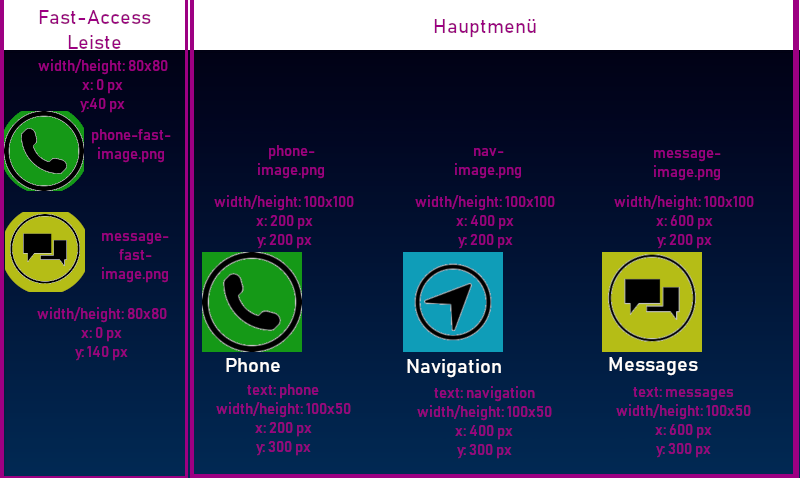
\includegraphics[width=0.9\linewidth]{figures/Styleguide_Rahmen.png}
  \captionof{figure}{Styleguide}
  \label{fig:Styleguide}
\end{center}

Auf Grundlage dieser Subtasks, scheint es weiterhin sinnvoll, den Testpersonen die Modellierung einen Startscreens eines Human Machine Interface der Automobilbranche als Testaufgabe modellieren zu lassen.
Hierfür ist es notwendig einen grafischen Styleguide zu erstellen an dem sich die Nutzer, wie aus ihrer täglichen Arbeit gewohnt, orientieren können.
Darüber hinaus ist es auch, für die Evaluierung der Tests, notwendig die Nutzer die exakt gleichen Aufgaben durchführen zu lassen.
Der, in \cref{fig:Styleguide} zu sehende, Styleguide zeigt einen Startscreen mit drei Bildern und Bildunterschriften im Hauptmenü und zwei Bildern in der Fast-Access-Leiste.
Für jedes dieser Elemente sind, die für den Modellierer relevanten Eigenschaften sichtbar, sowie die Namen der Bilder, wie sie auch in den Assets von EB GUIDE verwendet werden.
Diese Anmerkungen sind, innerhalb des Styleguides, alle in pink gehalten, um sie deutlich vom tatsächlichen Design abzugrenzen.
Wobei die Rahmen für das Hauptmenü und die Fast-Access Leiste ebenfalls der Orientierung dienen und zum Verständnis der, im Folgenden beschriebenen Arbeitsaufgabe notwendig sind.

Zusätzliche zu dieser grafischen Darstellung der Arbeitsaufgabe, wird noch eine textuelle Angabe erstellt, die für die Durchführung des Tests nötig ist.
Es werden insgesamt drei verschiedene Angaben erstellt, die in den Anhängen \ref{app:Aufgabe_Filter}, \ref{app:Aufgabe_Prototyp} und \ref{app:Aufgabe_Guide} zu finden sind.
Da ein Teil der Anpassungen implementiert und der andere Teil mithilfe eines Prototyps umgesetzt wurde ist es nötig den Test in zwei Teile aufzuspalten, weshalb auch zwei getrennte Angaben existieren.
In Testaufgabe \ref{app:Aufgabe_Filter} gilt es den implementierten Filter zu testen, weshalb die Nutzer hier aufgefordert werden, die drei Bilder für das Hauptmenü zu platzieren und mit Widget Feature Properties zu versehen.
Für diesen ersten Teil wird den Nutzern ein vorbereitetes Projekt mit den benötigten Assets zur Verfügung gestellt, um zu gewährleisten, dass Probanden mit einer identischen Ausgangssituation starten.
Es wird hier explizit nicht auf die implementierten Änderungen hingewiesen, da überprüft werden soll, ob diese von den Nutzern intuitiv benutzt wird.
Um jedoch zu gewährleisten, dass jeder Nutzer das Filterfeld theoretisch nutzen kann, wird darum geben die Bilder mit Widget Feature Properties zu versehen.

Für Aufgabe \ref{app:Aufgabe_Prototyp} ist es notwendig den Übergang in den Prototyp so nahtlos wie möglich zu gestalten und gleichzeitig wieder eine identische Ausgangssituation für alle Nutzer zu schaffen.
Das initiale Aussehen des Prototyps beinhaltet deshalb die drei eingefügten Bilder im Hauptmenü, entspricht also der Situation, mit der das vorherige Projekt in GUIDE von den Testpersonen verlassen wurde.
Da die Multiselektion eine Neuerung ist, die eher unwahrscheinlich selbstständig von den Nutzern entdeckt wird, wird hier zu Anfang darauf hingewiesen, dass der vorliegende Prototyp Multiselektion unterstützt.
Mit der Fast-Access Leiste, welche mithilfe von Templates modelliert werden soll, wird die Verlagerung der Funktion \glqq publish to template interface\grqq{} überprüft.
Ebenfalls wird in diesem Zuge darauf hingewiesen, dass nun auch Bilder mithilfe von Multiselektion in Templates eingefügt werden können, jedoch ohne genaue Erklärung, auf welche Art und Weise das funktioniert.
Abschließend sollen noch die Bilder und Labels positioniert und skaliert werden.
Es wird hier nicht mehr explizit auf die Multiselektion verwiesen, da herausgefunden werden soll, inwiefern die Probanden dies, nach der Information zu Beginn der Angabe, intuitiv für die restliche Aufgabe nutzen.

Die letzte Aufgabe \ref{app:Aufgabe_Guide} dient zur Erlangung der Vergleichswerte der Effizienz und wird deshalb in der unmodifizierten Version von GUIDE umgesetzt.
Da hier kein Übergang in den Prototyp notwendig ist, ist eine zusammenhängende Arbeitsaufgabe ausreichend.
Die Probanden sollen hier die identische Aufgabe durchführen und werden, angepasst an die beiden vorherigen Angaben, in der Nutzung von Templates eingeschränkt oder dazu aufgefordert.
Den Nutzern hier ein komplett freies Arbeiten zu gestatten ist nicht möglich, da möglichst identische Arbeitsschritte getätigt werden müssen um einen validen Vergleich anstellen zu können.

\section {Ergebnisse}
Die Anzahl der - in einem mit n Nutzern durchgeführten Test -  gefundenen Usabilityprobleme lässt sich laut Nielsen und Landauer nach folgender Formel berechnen.

\begin{center}
$\mathbf{N (1-(1- L ) ^n )}$ 
\end{center}

Wobei N der kompletten Anzahl der Usabilityprobleme im System entspricht und L der Anzahl der entdeckten Probleme nach dem Test mit einem Nutzer.
L entspricht hier im Durchschnitt 31\%, was zu der folgenden Grafik führt.  \cite{Nielsen.1993}

\begin{center}
  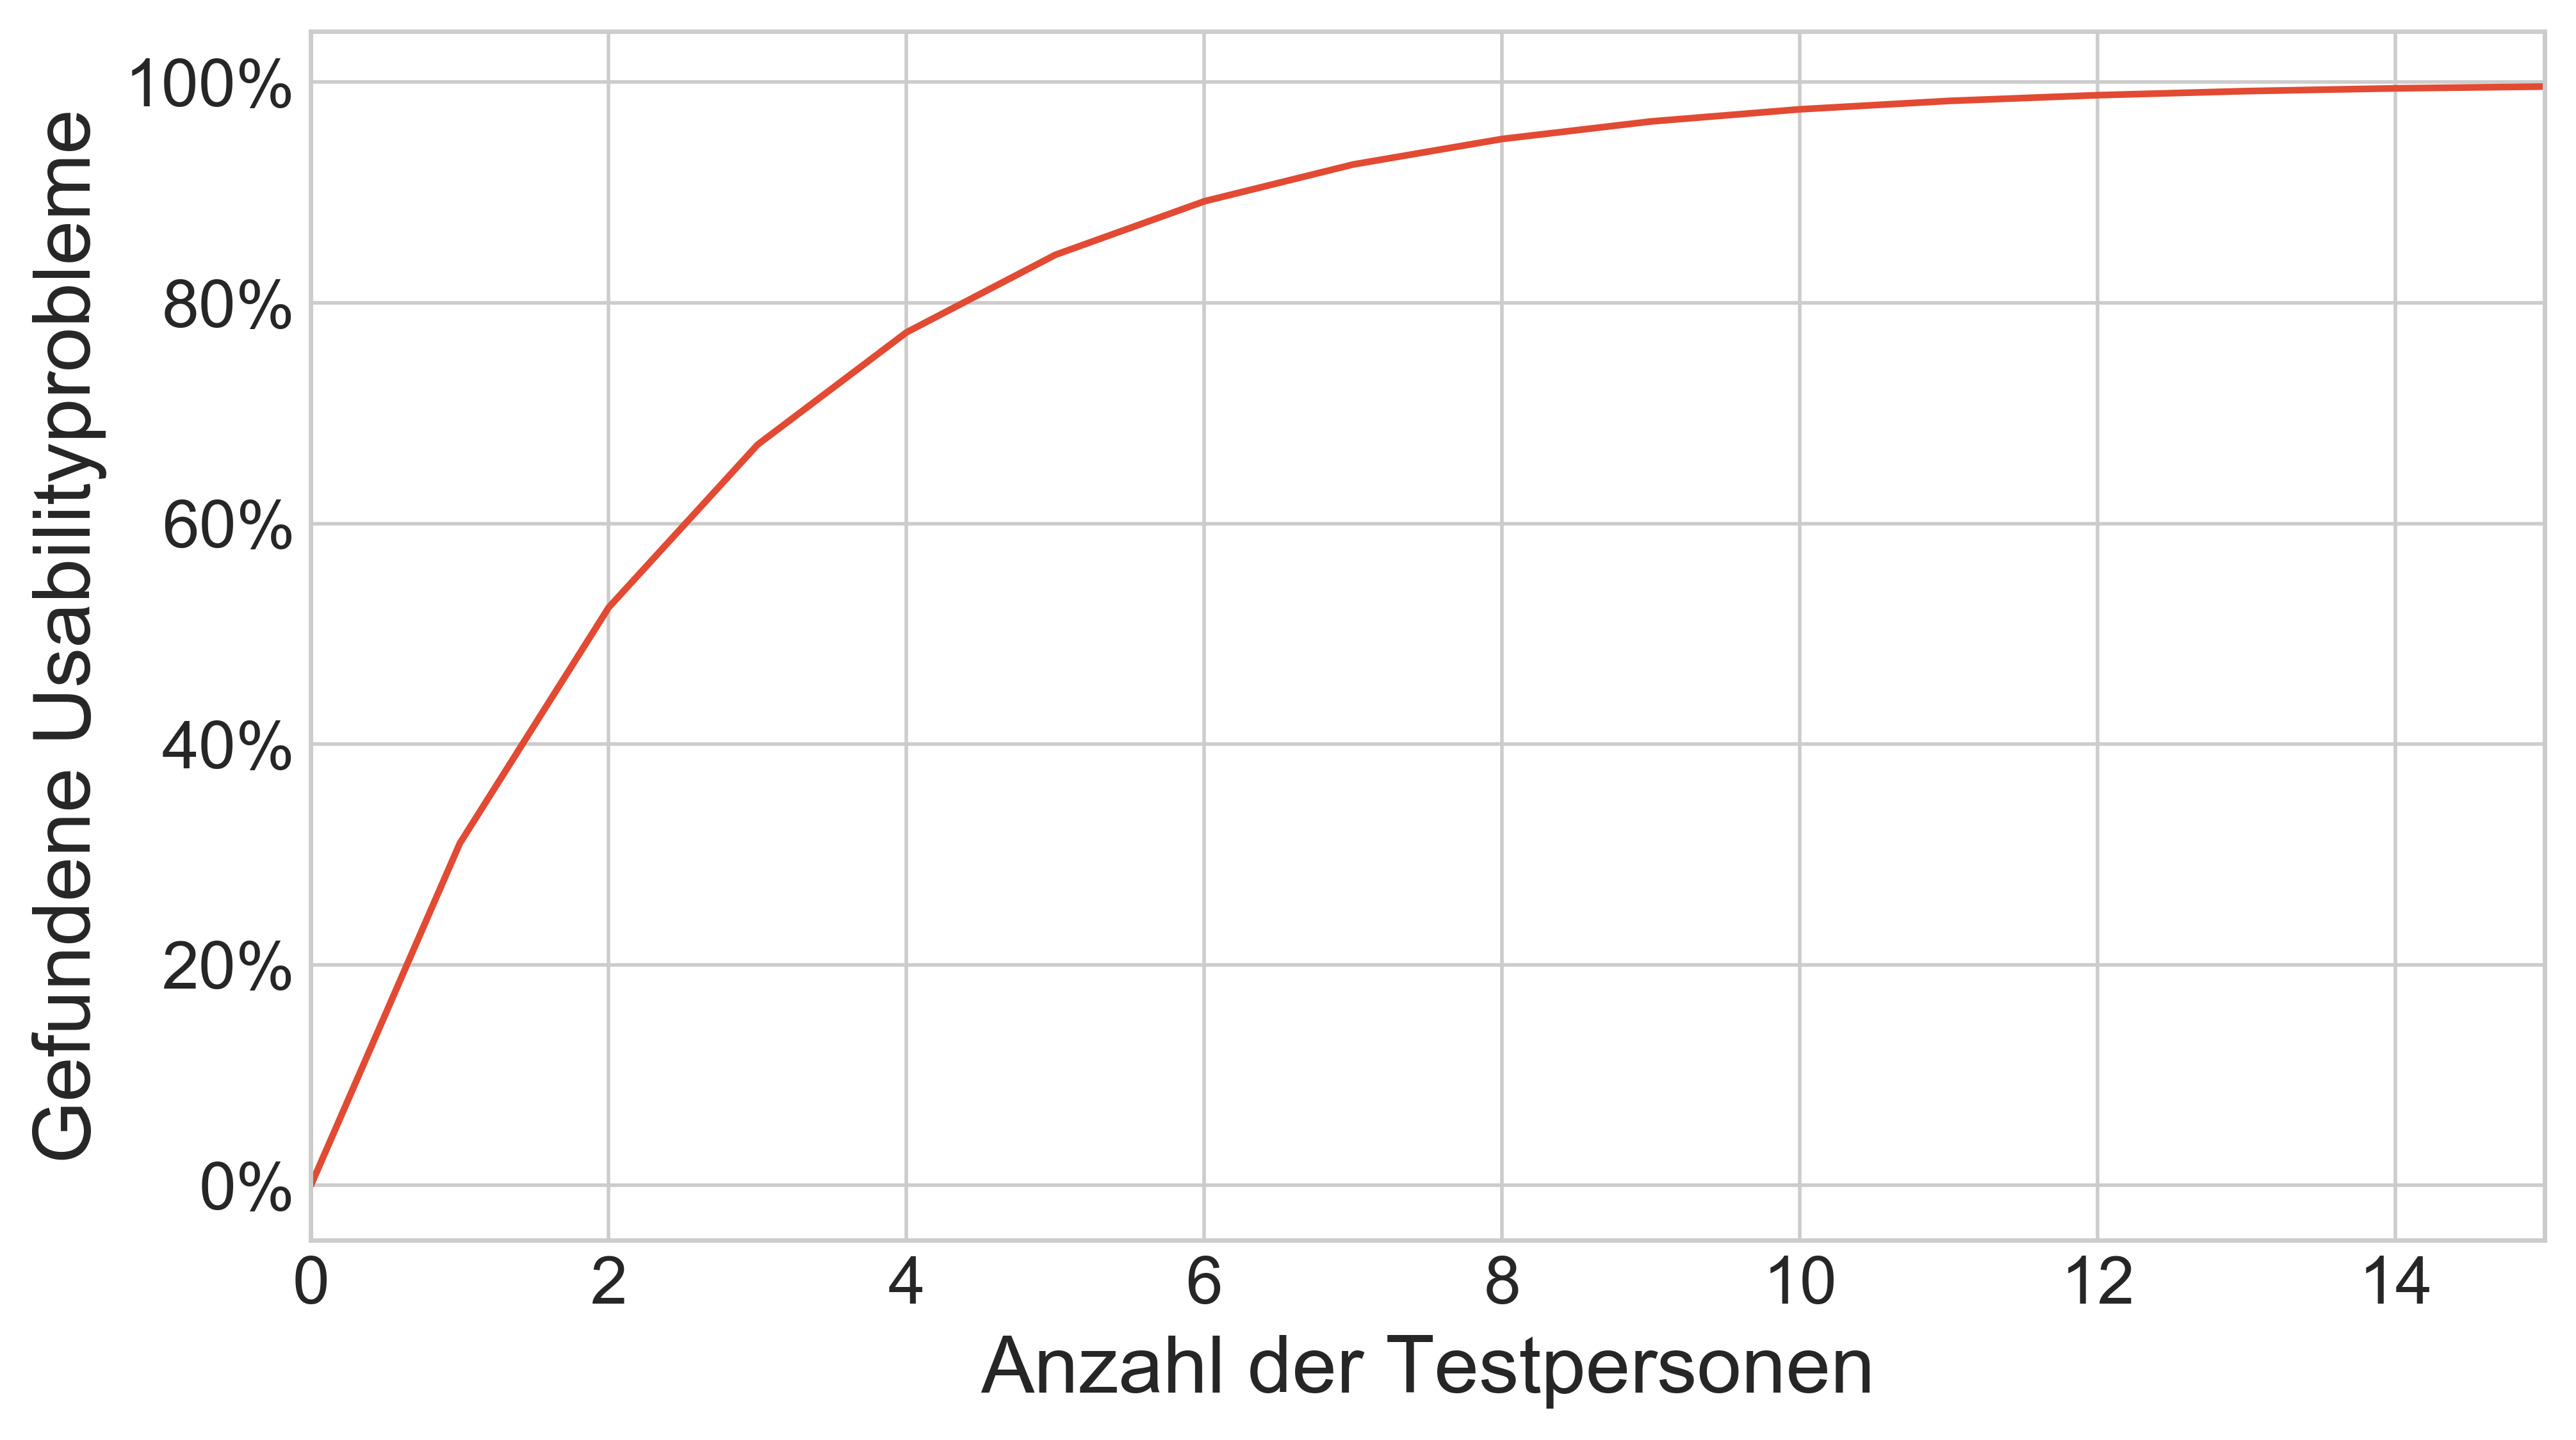
\includegraphics[width=0.7\linewidth]{figures/curve.png}
  \captionof{figure}{Aufdeckungsrate von Usabilityproblemen}
  \label{fig:curve}
\end{center}

Bei Betrachtung von \cref{fig:curve} wird deutlich, dass - solange mit keinem Nutzer getestet wurde - es auch keinen Aufschluss über die Usability Probleme eines Systems gibt.
Nach dem Test mit einem Nutzer, werden bereits fast ein Drittel der Schwächen aufgedeckt.
Wird der Test mit einem zweiten Nutzer durchgeführt, decken sich bereits einige der Beobachtungen, es werden aber durchaus noch neue Schwächen entdeckt und unterschiedliche Messergebnisse treten auf.
Je mehr Nutzer untersucht werden, desto häufiger decken sich die Beobachtungen und Messungen mit den Ergebnissen der bereits untersuchten Nutzer.\cite{.h}
Entgegen einer häufigen Annahme ist es also nicht unbedingt sinnvoll einen Usability Test mit einer möglichst großen Zahl an Testpersonen durchzuführen, da der Tester, ab einem gewissen Punkt, fast ausschließlich identische Probleme sehen und Messwerte erhalten wird.
Neue Informationen erhält man meist bis zur Untersuchung des fünften Nutzers, weshalb dies auch die optimale Anzahl an Probanden darstellt.

Wird nun aber, wie im Falle dieser Arbeit, eines der messbaren Usability Attribute verglichen, ist es nötig die Anzahl der Nutzer zu verdoppeln.
Es werden zwei verschiedene Versionen eines Systems verglichen, die jeweils von fünf Nutzer getestet werden.
Dadurch werden bei jedem System etwa 80\% bis 90\% der Schwächen aufgedeckt.
Bei der Messung der Attribute Effizienz und Fehlerrate kann ein repräsentativer Mittelwert gebildet werden.

Alternativ gäbe es die Möglichkeit den Test mit nur fünf Nutzern durchzuführen, was zu dem Vorteil führen würde, die Ergebnisse einer Person mit dem neuen und alten Interface direkt vergleichen zu können.
Allerdings würde hier die Problematik entstehen, dass der Nutzer die gleiche Arbeitsaufgabe doppelt durchführen würde, was zu einer Verfälschung der Ergebnisse führt, da die Angaben und Koordinaten der Objekte bereits bekannt sind.
Die Durchführung der identischen Arbeitsaufgabe ist jedoch dringend notwendig, um vergleichbare Werte zu erhalten.
Aus diesem Grund bevorzugt Nielsen die Messung mit der doppelten Anzahl an Probanden, statt Nutzern zweimal die gleiche Aufgabe durchführen zu lassen.\cite{.h}

Die im Folgenden dargestellten Ergebnisse wurden durch das Testen einer Gruppe aus zehn Personen erzeugt, die aus sechs Expertennutzern und vier Gelegenheitsnutzern besteht.
Zwar wäre eine 1:1 Zusammensetzung der Gruppe der Testpersonen wünschenswerter, firmenintern standen jedoch zum Zeitpunkt der Messung nicht mehr Personen zur Verfügung, weshalb es einen Expertennutzer mehr in der Testgruppe gibt.
Die Einstufung eines Expertennutzers wird dadurch definiert, dass die Person aktuell aktiv in einem Projekt mit EB GUIDE 6 arbeitet und dies auch schon seit mindestens 2 Monaten ununterbrochen tut.
Gelegenheitsnutzer sind all diejenigen, die zwischen dem Nutzen der Software immer mindestens 2 Wochen pausieren und eine einführende Schulung erfolgreich abgeschlossen haben.

Aus den gemessenen Werten wird jeweils ein Mittelwert gebildet, zusätzlich wird bei den Neuerungen untersucht welcher der möglichen Wege zur Problemlösung genutzt wird und welcher nicht.
Über die Fehlerrate kann ergänzend aufgedeckt werden, ob noch Verbesserungen am Design vorgenommen werden müssen.

\subsection{Ergebnisse überarbeitetes Interface}
Der Prototyp und der implementierte Filter werden demnach mit fünf Probanden getestet, welche sich aus drei Experten und zwei Gelegenheitsnutzern zusammensetzen.
Nach der Durchführung der Aufgabe werden den Nutzern noch zusätzliche Fragen zu ihrem Verhalten gestellt, welche in der folgenden Auswertung ebenfalls aufgeführt werden.

\paragraph{Widget Feature Properties}
Der Filter wird im Test von drei Probanden genutzt, die anderen beiden, jeweils ein Experte und ein Gelegenheitsnutzer, geben anschließend an die Funktion nicht gesehen zu haben.
Ein Nutzer wendet den Filter erst an, nachdem er zwei Menüs auf der Suche nach dem richtigen Feature ausgeklappt hat.
Er und die anderen Beiden geben anschließend an, den Filter nicht als Neuerung wahrgenommen zu haben, ihn jedoch intuitiv genutzt zu haben.

Die Auswahl eines Feature Properties dauert mithilfe des Filters durchschnittlich 2 Sekunden.
Zwei der Nutzer erzeugen eine Fehlerrate von 2 Fehlern bei der Auswahl.
Aus der Suche nach dem Scale Mode filtern die Probanden mit dem Wort \glqq Scal\grqq{}.
Dadurch taucht, wie in \cref{fig:Feature_Test} zu sehen, in der Ergebnissen zusätzlich zu dem Scale Mode das Feature Scaling auf, welches dann fälschlicherweise ausgewählt wird.

\begin{center}
  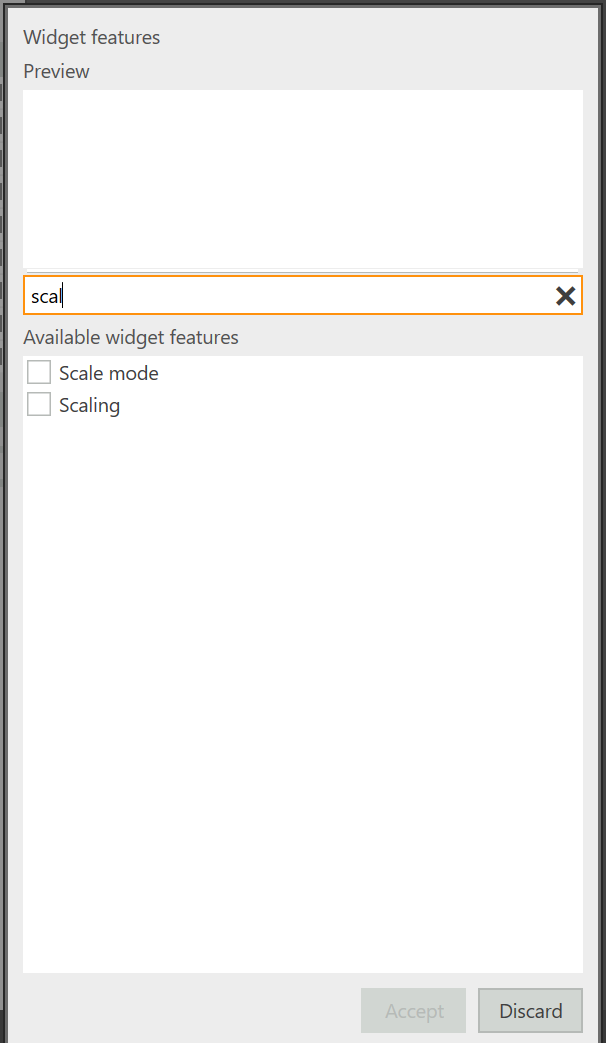
\includegraphics[scale= 0.6]{figures/Feature_Test.PNG}
  \captionof{figure}{Filterung nach Scale Mode}
  \label{fig:Feature_Test}
\end{center}

\paragraph{Publish to template interface}
Die Verlegung des Hotspots für die Funktion \glqq publish to template interface\grqq{} wird ebenfalls von drei, der fünf Probanden selbstständig gefunden, die alle benötigten Properties dadurch in durchschnittlich 4,6 sek publishen können.
Die neue Position wird von einem Experten und einem Gelegenheitsnutzer nicht entdeckt, jedoch - nach Aufklärung vonseiten des Testers - als nützlicher Shortcut eingestuft.
Bei den nötigen Klicks für die das Publishen der Objekteigenschaften wird eine Fehlerrate von 0 erzielt.

\paragraph{Multiselektion}
Für die Skalierung der drei Bilder des Hauptmenüs nutzen alle Probanden die Multiselektion und schließen den Vorgang in durchschnittlich 7,2 Sekunden ab, wobei ihnen keine Fehler unterlaufen.

Bei den Labels haben nur vier Testpersonen die Multiselektion in durchschnittlich 8 Sekunden mit einer Fehlerrate von 0 genutzt, der fünfte Nutzer hat, nach eigenen Aussagen, aus Gewohnheit jeden Text einzeln positioniert, obwohl vorher für die Bilder die Mehrfachselektion verwendet wurde.

Bei der Positionierung muss unterschieden werden, ob die Arbeitsaufgabe mithilfe der Alignment Actions oder mit einfacher Multiselektion gelöst wurde.

Ein Proband macht bei den Bildern Gebrauch von den Alignment Actions und schließt die Positionierung aller drei Bilder in 5 Sekunden ab.
Allerdings lässt sich hier eine Fehlerquelle beobachten.
Der Nutzer legt zuerst den Abstand zwischen den Objekten fest, vergisst jedoch das Ankerbild, an dem sich die anderen Bilder ausrichten, an die richtige Position zu setzen.
Nachdem dieses korrekt positioniert ist muss die Ausrichtung erneut durchgeführt werden.
Drei der anderen Nutzer haben die Alignment Actions bei den Bildern nicht gesehen, ein Vierter hat sie zwar wahrgenommen, hatte zu diesem Zeitpunkt die Bilder jedoch einzeln schon korrekt positioniert, dass er von der Nutzung abgesehen hat.

Bei den Labels nutzt dieser Proband die Alignment Actions, ebenso die Testperson, die diese Funktion auch bei den Bildern angewandt hat.
Dadurch kann die Positionierung hier in durchschnittlich 6 Sekunden abgeschlossen werden, es tritt jedoch ein identischer Fehler mit dem Ankerobjekt auf, was hier ebenfalls eine Fehlerrate von 1 ergibt.
Die Probanden die diese Funktion nicht nutzen, geben hierfür die gleichen Gründe an wie bei den Bildern.

Zusätzlich gibt es bei den Texten die Möglichkeit diese mithilfe der Alignment Actions an den Bildern auszurichten.
Auf die Idee ein Bild und den dazugehörigen Text gleichzeitig auszuwählen kommt jedoch keine der Testpersonen.
Dies ist darauf zurückzuführen, dass sich erst noch an die neuen Funktionen gewöhnt werden muss und die gleichzeitige Auswahl verschiedener Objekte zum aktuellen Zeitpunkt noch zu verwirrend ist.

Die Positionierung über normale Multiselektion wird bei den Bildern von vier Nutzern durchgeführt, wobei die identischen y-Koordinaten zusammen angepasst werden und danach die x-Koordinate für jedes Bild einzeln.
Mit diesem Vorgehen ist die Positionierung in durchschnittlich 3,5 Sekunden abgeschlossen und es werden zusätzlich keine Fehler gemessen.

Bei den Texten ist das Vorgehen für die Positionierung identisch, es treten ebenfalls keine Fehler auf und die durchschnittliche Zeitspanne beträgt 4,6 Sekunden.

Die Funktion \glqq Insert in Template\grqq{} wird von keinem der Nutzer entdeckt. Bei der abschließenden Befragung geben auch alle Probanden an, dass sie diese Funktion als nicht sinnvoll erachten.

\subsection{Ergebnisse altes Interface}
Um die Vergleichswerte zu erhalten wurde die Testaufgabe mit dem bestehenden Interface ebenfalls mit fünf Personen durchgeführt.
Die Zusammensetzung aus drei Experten und zwei Gelegenheitsnutzern ist hier identisch zu der Testgruppe des Prototypen.

\paragraph{Widget Feature Properties}
Da hier keine Filterfunktion zur Verfügung steht treten, wie zu erwarten, mehr Fehler bei den Nutzern auf.
Von den fünf Probanden begehen zwei Nutzer 2 Fehler und ein Nutzer 3 Fehler.
Die restlichen beiden Testpersonen finden das gewünschte Feature auf Anhieb, müssen hier jedoch einige Sekunden überlegen, weshalb bis zu Wahl des gewünschten Properties durchschnittlich 8,8 Sekunden vergehen.

\paragraph{Publish to template interface}
Die Funktion \glqq publish to template interface\grqq{} wird in der aktuellen Version von den Probanden in durchschnittlich 16 Sekunden abgeschlossen.
Eine Person erzeugt hier eine Fehlerrate von 1, indem sie nach dem Rechtsklick auf das Rechteck hinter dem zu verlinkenden Property zuerst die falsche Funktion auswählt.
Bei allen anderen Probanden lässt sich ebenfalls beobachten, dass sie kurz überlegen, welche der in \cref{fig:Template} zu sehenden Alternativen ausgewählt werden muss.
\begin{center}
  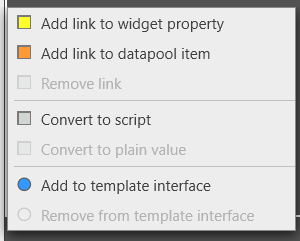
\includegraphics[scale= 0.8]{figures/Template.PNG}
  \captionof{figure}{Auswahlmöglichkeiten nach Rechtsklick auf Templateproperties }
  \label{fig:Template}
\end{center}

\paragraph{Positionieren/Skalieren ohne Multiselektion}
Das Skalieren und Positionieren der Texte und Bilder wird in der aktuellen Version von GUIDE  von den Nutzern meist so gelöst, dass ein Bild mit allen nötigen Features ausgestattet und dieses dann kopiert wird.
Anschließend ist es noch nötig die unterschiedlichen Eigenschaften der Kopien entsprechend der Spezifikation anzupassen.

Da bei der Skalierung die Werte nach dem Kopieren nicht mehr verändert werden müssen, kommen die Probanden hier auf eine durchschnittliche Arbeitszeit von 4,8 Sekunden, in der der Kopiervorgang bereits einberechnet ist.
Fehler treten hier nur auf, wenn die Probanden die Werte nicht händisch eingeben, sondern mit dem etwas komplizierteren Ansatz der Datapoolitems arbeiten.
Hierbei werden die Eigenschaften, wie Breite und Höhe mit einem Item verlinkt, dessen Wert sich an einer Stelle zentral anpassen lässt und alle verlinkten Objekte entsprechend verändert.
Fehler treten hierbei durch Verlinkung des falschen Datapoolitems oder der Eingabe des falschen Wertes auf.
Die Anzahl bemisst sich in diesem Testfall auf 2 Fehler bei einem Probanden, der diesen etwas komplizierteren Modellierungsansatz wählt.

Bei der Skalierung der Labels arbeitet keiner der Nutzer mit Datapoolitems, weshalb hier eine Fehlerrate von 0 erzeugt wird und der Vorgang für alle Texte in durchschnittlich 9 Sekunden abgeschlossen ist.

Für die Positionierung der Bilder und Labels müssen die Eigenschaften der kopierten Elemente angepasst werden.
Dies geschieht für erstere in 8,5 Sekunden, bei den Labels dauert es durchschnittlich 10,8 Sekunden.
Hierbei tritt bei den Bildern ebenfalls ein Fehler bei der Arbeit mit den Datapoolitems auf, bei den Texten beläuft sich die Fehlerrate bei allen Nutzern auf 0.

\subsection{Vergleich und Interpretation}Auf Grundlage der gemessenen Daten kann nun ein direkter Vergleich zwischen dem bestehenden und dem überarbeiteten Interface von EB GUIDE getätigt werden.
Weiterhin können Beobachtungen über die Nutzung der Ergänzungen interpretiert werden und anhand der Messwerte evaluiert werden, ob die definierten quantitativen Benutzeranforderungen erfüllt wurden.

\paragraph{Widget Feature Properties}
Mithilfe des Filters gelingt es den Probanden 8,8 Sekunden schneller das gewünschte Feature Property zu finden, wodurch die Anforderung an die Effizienz erfüllt ist.
Die angestrebte Fehlerrate von 0 kann jedoch aktuell noch nicht erzielt werden.
Die Fehler können sich vermutlich darauf zurückführen lassen, dass die Nutzer an die übergeordneten Kategorien gewöhnt sind und sich deshalb nicht sicher sind, ob sie Scaling oder Scale Mode auswählen müssen.
Hier bestünde die Möglichkeit in einer weiteren Iteration zu testen ob sich die Fehleranzahl wieder verringert, wenn die Kategorien während des Filterns eingeblendet bleiben.

\paragraph{Publish to template interface}
Die neue Position der Publish Funktion wurde zwar nicht von allen Nutzern selbstständig gefunden, wurde jedoch im Nachhinein von allen als sinnvoll eingestuft.
Die erreichte Fehlerrate von 0 stellt hier eine Verbesserung dar, da bei der jetzigen Implementierung teilweise falsche Optionen ausgewählt werden und die Nutzer lange überlegen müssen.
Zusätzlich schließen die Probanden ihr Vorgehen 11,4 Sekunden schneller ab, was sich auf den fehlenden Rechtsklick zurückführen lässt.
Damit sind beide Benutzeranforderungen für diese Funktion erfüllt.
Trotzdem kann die neue Position die vorherige nicht in Gänze ersetzen, da es für Erstnutzer nicht möglich ist, die Funktion des Klicks zu erkennen.
Daher bietet sich eine Kombination der bisherigen Implementierung und der Neuerung an.
Nutzer, die sich der Funktion bewusst sind, können den schnelleren Weg über Klick auf den Kreis wählen, Modellierer die sich noch mit der Funktionsweise von GUIDE vertraut machen, können die bisherige Variante mit dem erklärenden Text wählen.

\paragraph{Multiselektion}
Die Funktion \glqq Insert in Template\grqq{} wurde von keinem der Probanden benutzt und auch bei einer nachträglichen Befragung als nicht hilfreich eingestuft.
Deshalb erscheint es hier sinnvoll diese Funktion nicht weiterzuverfolgen.

Die Alignment Actions beschleunigen die Positionierung der Bilder und der Texte, bringen jedoch aktuell noch eine höhere Fehlerrate mit sich, als die bis jetzt übliche Art der Positionierung.
Die begangenen Fehler lassen sich jedoch auch darauf zurückführen, dass diese Funktion in GUIDE eine komplett neue und daher ungewohnte Ergänzung bietet.
Neue Funktionen müssen erst getestet und verstanden werden.
Die falsche Ausführungsreihenfolge ist ein Fehler, der vermutlich nur zu Anfang und nicht mehr bei regelmäßigem Gebrauch auftritt.
Diese Möglichkeiten zu erweitern und fortlaufend zu untersuchen würde sich also lohnen.
Auch das Alignment von Text an Bildern sollte, zumindest für eine weitere Iteration, weiter verfolgt werden, um herauszufinden, ob die Nutzer, da sie nun von dieser Funktionalität wissen, diese auch benutzen.
Die Anforderung der höheren Effizienz wird durch die Alignment Actions demnach bereits erfüllt, in Bezug auf die Fehlerrate sind jedoch noch Nachbesserungen erforderlich.

Die Positionierung der Elemente ohne Alignment Actions, sondern nur mit Multiselektion, hat innerhalb des durchgeführten Tests  mit 3,5 Sekunden zeitlich am besten abgeschnitten, auch wurden hier keine Fehler durch die Nutzer begangen.
Gleichzeitige Anpassung von Properties scheint sowohl zeitlich sinnvoll, als auch für den Nutzer intuitiv zu verlaufen und erfüllt zudem die formulierten Benutzeranforderungen.

Bei der Skalierung der Bilder bietet die Multiselektion, auf den ersten Blick, keinen zeitlichen Vorteil.
Es gilt jedoch zu bedenken, dass im Testfall nur drei Bilder vorhanden sind, der Kopiervorgang dieser Bilder also kein großes zeitliches Gewicht hat.
Beinhaltet eine Spezifikation jedoch beispielsweise zehn, statt nur drei Bilder, geht durch den Kopiervorgang bereits mehr Zeit verloren.
Den Ansatz, die Objekte zu kopieren und dann entsprechend anzupassen, haben die Nutzer nur bei den Bildern, jedoch nicht bei den Texten verfolgt.
Deshalb lässt sich bei den Messwerten innerhalb des Prototyps eine zeitliche Verbesserung gegenüber der bisherigen Version verzeichnen.
Da sich die Multiselektion für die Positionierung bereits als Mehrwert erwiesen hat, ist es sinnvoll die gleichzeitige Anpassung aller Properties bei Mehrfachselektion zu ermöglichen.
Es würde den Nutzer irritieren, wenn nur gewisse Eigenschaften gleichzeitig anpassbar wären, weshalb es sinnvoll ist, auch weiterhin width und height der Objekte zusammen anpassen zu können.
In weiteren Iteration wäre es hier jedoch sinnvoll zu untersuchen, ob bei größeren Projekten tatsächlich ein zeitlicher Mehrwert eintritt, da dies hier lediglich vermutet wird.
Die Benutzeranforderungen sind, im Bezug auf die Skalierung der Objekte, dementsprechend noch nicht komplett erfüllt.
Die Fehlerrate beläuft sich zwar weiterhin auf 0, allerdings ist ein Mehrwert im Bezug auf die Effizienz noch nicht sichergestellt.

\section {Ausblick}
Die vorliegenden Ergebnisse werden auf Grundlage einer Iteration des Human Centered Design Process erlangt.
Je nachdem, ob nach dieser Iteration die Benutzeranforderungen erfüllt sind, ist es notwendig das Design anzupassen und nochmals zu evaluieren oder es als abgeschlossen zu betrachten und zur Implementierung überzugehen.

Wie im vorherigen Abschnitt bereits festgehalten erfüllt die Filterfunktion noch nicht alle Anforderungen und bedarf in Bezug auf die Fehlerrate noch einer Nachbesserung.
Diese gilt es in einem weiteren Test erneut zu evaluieren.

Die neue Position der Funktion \glqq publish to template interface\grqq{} erfüllt alle definierten Bedingungen und kann deshalb, zusätzlich zur bestehenden Funktion, implementiert werden.

Die Funktionen der Multiselektion gilt es an diesem Punkt differenziert zu betrachten.
Da diese Ergänzung komplett neu in EB GUIDE sind, gibt es hier noch viele Möglichkeiten und Funktionen, die hinzugefügt und evaluiert werden können.
Das gleichzeitige Anpassen von Eigenschaften, wie der Position und Skalierung von Objekten, hat sich im Rahmen dieser Iteration bereits als nützlich erwiesen und kann ebenfalls implementiert werden, da herausgefunden wurde, dass die Modellierer diese Funktion auch nutzen.
Dadurch wird eine Grundlage für weitere Interaktionsmöglichkeiten dieser Art gelegt.
So ist es beispielsweise üblich die Eigenschaften, die nun gemeinsam anpassbar sind, mit Datapoolitems zu verlinken.
Bei den Befragungen nach dem Tests äußern hier einige der Nutzer den Wunsch diese Verlinkung ebenfalls, mithilfe der Multiselektion durchführen zu können, was für eine weitere Iteration im Prototyp ergänzt und evaluiert werden kann.
Zusätzlich wird angegeben, dass über dem Propertie Panel angezeigt werden soll, welche Objekte aktuell zusammen ausgewählt sind, da dies bis jetzt nur im View erkennbar ist.

Da bei den durchgeführten Tests deutlich wird, dass die Nutzer sich für die Alignment Actions interessieren, kann nun in folgenden Iterationen noch eine Verbesserung und Erweiterung der Funktionalitäten angestrebt werden.
Für diesen Test war der Prototyp so ausgelegt, dass bereits bekannt war, welches der drei Bilder des Hauptmenüs links, rechts und in der Mitte liegt.
Dadurch hat sich die Anordnung, durch einen Klick auf den Button, automatisch an die Spezifikation angepasst.
Für tatsächliche Arbeitsabläufe ist dies nicht der Fall, weshalb es für den Nutzer möglich sein muss, anzugeben in welcher Anordnung die Bilder platziert werden sollen.
Dies wäre zum Beispiel dadurch umsetzbar, dass der Nutzer ein Objekt als Ausrichtungspunkt deklarieren kann.

Die Multiselektion bietet also noch viele Möglichkeiten, die in weiteren Durchführungen des Human Centered Design Process den Prototyp zu ergänzen und die neuen Funktionen zu evaluieren, die Funktion \glqq Insert in Template\grqq{} gilt es jedoch zum aktuellen Zeitpunkt zu verwerfen.